\chapter{Positioning}\label{cha:position}

\section{Introduction}

This chapter discusses position, particularly how facets are laid out on
a page, and how coordinate systems within a panel work. There are four
components that control position. You have already learned about two of
them that work within a facet: \index{Positioning}

\begin{itemize}
\item
  \textbf{Position adjustments} adjust the position of overlapping
  objects within a layer. These are most useful for bar and other
  interval geoms, but can be useful in other situations
  (\hyperref[sec:position]{link to section}).
\item
  \textbf{Position scales} control how the values in the data are mapped
  to positions on the plot (\hyperref[sub:scale-position]{link to
  section}).
\end{itemize}

This chapter will describe the other two components and show you how all
four pieces fit together:

\begin{itemize}
\item
  \textbf{Facetting} is a mechanism for automatically laying out
  multiple plots on a page. It splits the data into subsets, and then
  plots each subset in a different panel. Such plots are often called
  small multiples or trellis graphics (\hyperref[sec:facetting]{link to
  section}).
\item
  \textbf{Coordinate systems} control how the two independent position
  scales are combined to create a 2d coordinate system. The most common
  coordinate system is Cartesian, but other coordinate systems can be
  useful in special circumstances (\hyperref[sec:coord]{link to
  section}).
\end{itemize}

\hyperdef{}{sec:facetting}{\section{Facetting}\label{sec:facetting}}

You first encountered facetting in
\hyperref[sec:qplot-facetting]{getting started}. Facetting generates
small multiples each showing a different subset of the data. Small
multiples are a powerful tool for exploratory data analysis: you can
rapidly compare patterns in different parts of the data and see whether
they are the same or different. This section will discuss how you can
fine-tune facets, particularly the way in which they interact with
position scales. \index{Facetting} \index{Positioning!facetting}

There are three types of facetting:

\begin{itemize}
\item
  \texttt{facet\_null()}: a single plot, the default.
  \indexf{facet\_null}
\item
  \texttt{facet\_wrap()} ``wraps'' a 1d ribbon of panels into 2d.
\item
  \texttt{facet\_grid()}: produces a 2d grid of panels defined by
  variables which form the rows and columns.
\end{itemize}

The difference between \texttt{facet\_wrap()} and \texttt{facet\_grid()}
are illustrated in Figure \ref{fig:facet-sketch}.

\begin{figure}[htbp]
  \centering
    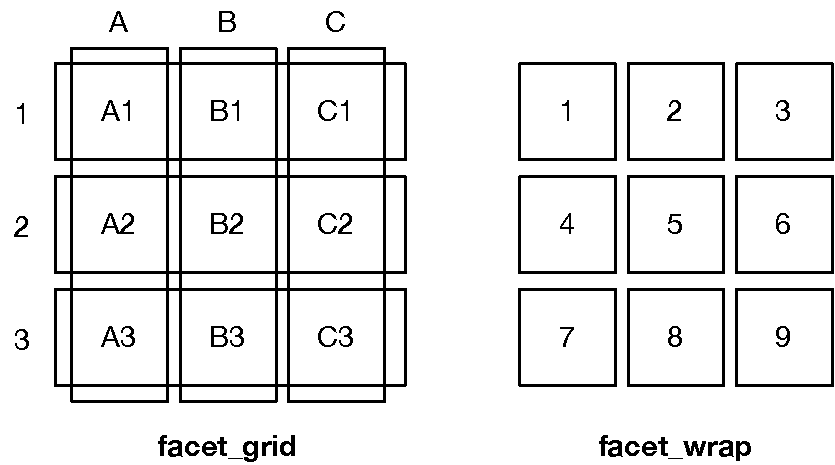
\includegraphics[width=0.75\linewidth]{diagrams/position-facets}
  \caption{A sketch illustrating the difference between the two facetting systems. \texttt{facet\_grid()} (left) is fundamentally 2d, being made up of two independent components. \texttt{facet\_wrap()} (right) is 1d, but wrapped into 2d to save space.}
  \label{fig:facet-sketch}
\end{figure}

Faceted plots have the capability to fill up a lot of space, so for this
chapter we will use a subset of the mpg dataset that has a manageable
number of levels: three cylinders (4, 6, 8), two types of drive train (4
and f), and six classes.

\begin{Shaded}
\begin{Highlighting}[]
\NormalTok{mpg2 <-}\StringTok{ }\KeywordTok{subset}\NormalTok{(mpg, cyl !=}\StringTok{ }\DecValTok{5} \NormalTok{&}\StringTok{ }\NormalTok{drv %in%}\StringTok{ }\KeywordTok{c}\NormalTok{(}\StringTok{"4"}\NormalTok{, }\StringTok{"f"}\NormalTok{) &}\StringTok{ }\NormalTok{class !=}\StringTok{ "2seater"}\NormalTok{)}
\end{Highlighting}
\end{Shaded}

\subsection{Facet wrap}\label{sub:facet-wrap}

\texttt{facet\_wrap()} makes a long ribbon of panels (generated by any
number of variables) and wraps it into 2d. This is useful if you have a
single variable with many levels and want to arrange the plots in a more
space efficient manner. \index{Facetting!wrapped} \indexf{facet\_wrap}
\indexc{\textasciitilde}

You can control how the ribbon is wrapped into a grid with
\texttt{ncol}, \texttt{nrow}, \texttt{as.table} and \texttt{dir}.
\texttt{ncol} and \texttt{nrow} control how many rows and columns (you
only need to set one). \texttt{as.table} controls whether the facets are
laid out like a table (\texttt{TRUE}), with highest values at the
bottom-right, or a plot (\texttt{FALSE}), with the highest values at the
top-right. \texttt{dir} controls the direction of wrap:
\textbf{h}orizontal or \textbf{v}ertical.

\begin{Shaded}
\begin{Highlighting}[]
\NormalTok{base <-}\StringTok{ }\KeywordTok{ggplot}\NormalTok{(mpg2, }\KeywordTok{aes}\NormalTok{(displ, hwy)) +}\StringTok{ }
\StringTok{  }\KeywordTok{geom_blank}\NormalTok{() +}\StringTok{ }
\StringTok{  }\KeywordTok{xlab}\NormalTok{(}\OtherTok{NULL}\NormalTok{) +}\StringTok{ }
\StringTok{  }\KeywordTok{ylab}\NormalTok{(}\OtherTok{NULL}\NormalTok{)}

\NormalTok{base +}\StringTok{ }\KeywordTok{facet_wrap}\NormalTok{(~class, }\DataTypeTok{ncol =} \DecValTok{3}\NormalTok{)}
\NormalTok{base +}\StringTok{ }\KeywordTok{facet_wrap}\NormalTok{(~class, }\DataTypeTok{ncol =} \DecValTok{3}\NormalTok{, }\DataTypeTok{as.table =} \OtherTok{FALSE}\NormalTok{)}
\end{Highlighting}
\end{Shaded}

\begin{figure}[H]
  \includegraphics[width=0.5\linewidth]{_figures/position/unnamed-chunk-1-1}%
  \includegraphics[width=0.5\linewidth]{_figures/position/unnamed-chunk-1-2}
\end{figure}

\begin{Shaded}
\begin{Highlighting}[]
\NormalTok{base +}\StringTok{ }\KeywordTok{facet_wrap}\NormalTok{(~class, }\DataTypeTok{nrow =} \DecValTok{3}\NormalTok{)}
\NormalTok{base +}\StringTok{ }\KeywordTok{facet_wrap}\NormalTok{(~class, }\DataTypeTok{nrow =} \DecValTok{3}\NormalTok{, }\DataTypeTok{dir =} \StringTok{"v"}\NormalTok{)}
\end{Highlighting}
\end{Shaded}

\begin{figure}[H]
  \includegraphics[width=0.5\linewidth]{_figures/position/unnamed-chunk-2-1}%
  \includegraphics[width=0.5\linewidth]{_figures/position/unnamed-chunk-2-2}
\end{figure}

\subsection{Facet grid}

\texttt{facet\_grid()} lays out plots in a 2d grid, as defined by a
formula: \index{Facetting!grid} \indexf{facet\_grid}

\begin{itemize}
\item
  \texttt{.\ \textasciitilde{}\ a} spreads the values of \texttt{a}
  across the columns. This direction\\
   facilitates comparisons of y position, because the vertical scales
  are aligned.

\begin{Shaded}
\begin{Highlighting}[]
\NormalTok{base +}\StringTok{ }\KeywordTok{facet_grid}\NormalTok{(. ~}\StringTok{ }\NormalTok{cyl)}
\end{Highlighting}
\end{Shaded}

  \begin{figure}[H]
    \centering
    \includegraphics[width=0.75\linewidth]{_figures/position/grid-v-1}
  \end{figure}
\item
  \texttt{b\ \textasciitilde{}\ .} spreads the values of \texttt{b} down
  the rows. This direction facilitates comparison of x position because
  the horizontal scales are aligned. This makes it particularly useful
  for comparing distributions.

\begin{Shaded}
\begin{Highlighting}[]
\NormalTok{base +}\StringTok{ }\KeywordTok{facet_grid}\NormalTok{(drv ~}\StringTok{ }\NormalTok{.)}
\end{Highlighting}
\end{Shaded}

  \begin{figure}[H]
    \centering
    \includegraphics[width=0.3\linewidth]{_figures/position/mpg2-h-1}
  \end{figure}
\item
  \texttt{a\ \textasciitilde{}\ b} spreads \texttt{a} across columns and
  \texttt{b} down rows. You'll usually want to put the variable with the
  greatest number of levels in the columns, to take advantage of the
  aspect ratio of your screen.

\begin{Shaded}
\begin{Highlighting}[]
\NormalTok{base +}\StringTok{ }\KeywordTok{facet_grid}\NormalTok{(drv ~}\StringTok{ }\NormalTok{cyl)}
\end{Highlighting}
\end{Shaded}

  \begin{figure}[H]
    \centering
    \includegraphics[width=0.75\linewidth]{_figures/position/grid-vh-1}
  \end{figure}
\end{itemize}

You can use multiple variables in the rows or columns, by ``adding''
them together, e.g. \texttt{a\ +\ b\ \textasciitilde{}\ c\ +\ d}.
Variables appearing together on the rows or columns are nested in the
sense that only combinations that appear in the data will appear in the
plot. Variables that are specified on rows and columns will be crossed:
all combinations will be shown, including those that didn't appear in
the original dataset: this may result in empty panels.

\subsection{Controlling scales}\label{sub:controlling-scales}

For both \texttt{facet\_wrap()} and \texttt{facet\_grid()} you can
control whether the position scales are the same in all panels (fixed)
or allowed to vary between panels (free) with the \texttt{scales}
parameter: \index{Facetting!interaction with scales}
\index{Scales!interaction with facetting}
\index{Facetting!controlling scales}

\begin{itemize}
\tightlist
\item
  \texttt{scales\ =\ "fixed"}: x and y scales are fixed across all
  panels.
\item
  \texttt{scales\ =\ "free\_x"}: the x scale is free, and the y scale is
  fixed.
\item
  \texttt{scales\ =\ "free\_y"}: the y scale is free, and the x scale is
  fixed.
\item
  \texttt{scales\ =\ "free"}: x and y scales vary across panels.
\end{itemize}

\texttt{facet\_grid()} imposes an additional constraint on the scales:
all panels in a column must have the same x scale, and all panels in a
row must have the same y scale. This is because each column shares an x
axis, and each row shares a y axis.

Fixed scales make it easier to see patterns across panels; free scales
make it easier to see patterns within panels.

\begin{Shaded}
\begin{Highlighting}[]
\NormalTok{p <-}\StringTok{ }\KeywordTok{ggplot}\NormalTok{(mpg2, }\KeywordTok{aes}\NormalTok{(cty, hwy)) +}\StringTok{ }
\StringTok{  }\KeywordTok{geom_abline}\NormalTok{() +}
\StringTok{  }\KeywordTok{geom_jitter}\NormalTok{(}\DataTypeTok{width =} \FloatTok{0.1}\NormalTok{, }\DataTypeTok{height =} \FloatTok{0.1}\NormalTok{) }
\NormalTok{p +}\StringTok{ }\KeywordTok{facet_wrap}\NormalTok{(~cyl)}
\end{Highlighting}
\end{Shaded}

\begin{figure}[H]
  \centering
  \includegraphics[width=0.75\linewidth]{_figures/position/fixed-vs-free-1}%
\end{figure}

\begin{Shaded}
\begin{Highlighting}[]
\NormalTok{p +}\StringTok{ }\KeywordTok{facet_wrap}\NormalTok{(~cyl, }\DataTypeTok{scales =} \StringTok{"free"}\NormalTok{)}
\end{Highlighting}
\end{Shaded}

\begin{figure}[H]
  \centering
  \includegraphics[width=0.75\linewidth]{_figures/position/fixed-vs-free-2}
\end{figure}

Free scales are also useful when we want to display multiple times
series that were measured on different scales. To do this, we first need
to change from `wide' to `long' data, stacking the separate variables
into a single column. An example of this is shown below with the long
form of the \texttt{economics} data, and the topic is discussed in more
detail in \hyperref[sec:spread-gather]{converting data from wide to
long}. \index{Data!economics\_long@\texttt{economics\_long}}

\begin{Shaded}
\begin{Highlighting}[]
\NormalTok{economics_long}
\CommentTok{#> Source: local data frame [2,870 x 4]}
\CommentTok{#> Groups: variable [5]}
\CommentTok{#> }
\CommentTok{#>          date variable value  value01}
\CommentTok{#>        (date)   (fctr) (dbl)    (dbl)}
\CommentTok{#> 1  1967-07-01      pce   507 0.000000}
\CommentTok{#> 2  1967-08-01      pce   510 0.000266}
\CommentTok{#> 3  1967-09-01      pce   516 0.000764}
\CommentTok{#> 4  1967-10-01      pce   513 0.000472}
\CommentTok{#> 5  1967-11-01      pce   518 0.000918}
\CommentTok{#> 6  1967-12-01      pce   526 0.001579}
\CommentTok{#> ..        ...      ...   ...      ...}
\KeywordTok{ggplot}\NormalTok{(economics_long, }\KeywordTok{aes}\NormalTok{(date, value)) +}\StringTok{ }
\StringTok{  }\KeywordTok{geom_line}\NormalTok{() +}\StringTok{ }
\StringTok{  }\KeywordTok{facet_wrap}\NormalTok{(~variable, }\DataTypeTok{scales =} \StringTok{"free_y"}\NormalTok{, }\DataTypeTok{ncol =} \DecValTok{1}\NormalTok{)}
\end{Highlighting}
\end{Shaded}

\begin{figure}[H]
  \centering
  \includegraphics[width=0.75\linewidth]{_figures/position/time-1}
\end{figure}

\texttt{facet\_grid()} has an additional parameter called
\texttt{space}, which takes the same values as \texttt{scales}. When
space is ``free'', each column (or row) will have width (or height)
proportional to the range of the scale for that column (or row). This
makes the scaling equal across the whole plot: 1 cm on each panel maps
to the same range of data. (This is somewhat analogous to the `sliced'
axis limits of lattice.) For example, if panel a had range 2 and panel b
had range 4, one-third of the space would be given to a, and two-thirds
to b. This is most useful for categorical scales, where we can assign
space proportionally based on the number of levels in each facet, as
illustrated below.

\begin{Shaded}
\begin{Highlighting}[]
\NormalTok{mpg2$model <-}\StringTok{ }\KeywordTok{reorder}\NormalTok{(mpg2$model, mpg2$cty)}
\NormalTok{mpg2$manufacturer <-}\StringTok{ }\KeywordTok{reorder}\NormalTok{(mpg2$manufacturer, -mpg2$cty)}
\KeywordTok{ggplot}\NormalTok{(mpg2, }\KeywordTok{aes}\NormalTok{(cty, model)) +}\StringTok{ }
\StringTok{  }\KeywordTok{geom_point}\NormalTok{() +}\StringTok{ }
\StringTok{  }\KeywordTok{facet_grid}\NormalTok{(manufacturer ~}\StringTok{ }\NormalTok{., }\DataTypeTok{scales =} \StringTok{"free"}\NormalTok{, }\DataTypeTok{space =} \StringTok{"free"}\NormalTok{) +}
\StringTok{  }\KeywordTok{theme}\NormalTok{(}\DataTypeTok{strip.text.y =} \KeywordTok{element_text}\NormalTok{(}\DataTypeTok{angle =} \DecValTok{0}\NormalTok{))}
\end{Highlighting}
\end{Shaded}

\begin{figure}[H]
  \centering
  \includegraphics[width=0.75\linewidth]{_figures/position/discrete-free-1}
\end{figure}

\subsection{Missing facetting
variables}\label{sub:missing-facetting-columns}

If you are using facetting on a plot with multiple datasets, what
happens when one of those datasets is missing the facetting variables?
This situation commonly arises when you are adding contextual
information that should be the same in all panels. For example, imagine
you have a spatial display of disease faceted by gender. What happens
when you add a map layer that does not contain the gender variable? Here
ggplot will do what you expect: it will display the map in every facet:
missing facetting variables are treated like they have all values.
\index{Facetting!missing data}

Here's a simple example. Note how the single red point from \texttt{df2}
appears in both panels.

\begin{Shaded}
\begin{Highlighting}[]
\NormalTok{df1 <-}\StringTok{ }\KeywordTok{data.frame}\NormalTok{(}\DataTypeTok{x =} \DecValTok{1}\NormalTok{:}\DecValTok{3}\NormalTok{, }\DataTypeTok{y =} \DecValTok{1}\NormalTok{:}\DecValTok{3}\NormalTok{, }\DataTypeTok{gender =} \KeywordTok{c}\NormalTok{(}\StringTok{"f"}\NormalTok{, }\StringTok{"f"}\NormalTok{, }\StringTok{"m"}\NormalTok{))}
\NormalTok{df2 <-}\StringTok{ }\KeywordTok{data.frame}\NormalTok{(}\DataTypeTok{x =} \DecValTok{2}\NormalTok{, }\DataTypeTok{y =} \DecValTok{2}\NormalTok{)}

\KeywordTok{ggplot}\NormalTok{(df1, }\KeywordTok{aes}\NormalTok{(x, y)) +}\StringTok{ }
\StringTok{  }\KeywordTok{geom_point}\NormalTok{(}\DataTypeTok{data =} \NormalTok{df2, }\DataTypeTok{colour =} \StringTok{"red"}\NormalTok{, }\DataTypeTok{size =} \DecValTok{2}\NormalTok{) +}\StringTok{ }
\StringTok{  }\KeywordTok{geom_point}\NormalTok{() +}\StringTok{ }
\StringTok{  }\KeywordTok{facet_wrap}\NormalTok{(~gender)}
\end{Highlighting}
\end{Shaded}

\begin{figure}[H]
  \centering
  \includegraphics[width=0.75\linewidth]{_figures/position/unnamed-chunk-3-1}
\end{figure}

This technique is particularly useful when you add annotations to make
it easier to compare between facets, as shown in the next section.

\subsection{Grouping vs.~facetting}\label{sub:group-vs-facet}

Facetting is an alternative to using aesthetics (like colour, shape or
size) to differentiate groups. Both techniques have strengths and
weaknesses, based around the relative positions of the subsets.
\index{Facetting!vs. grouping} \index{Grouping!vs. facetting} With
facetting, each group is quite far apart in its own panel, and there is
no overlap between the groups. This is good if the groups overlap a lot,
but it does make small differences harder to see. When using aesthetics
to differentiate groups, the groups are close together and may overlap,
but small differences are easier to see.

\begin{Shaded}
\begin{Highlighting}[]
\NormalTok{df <-}\StringTok{ }\KeywordTok{data.frame}\NormalTok{(}
  \DataTypeTok{x =} \KeywordTok{rnorm}\NormalTok{(}\DecValTok{120}\NormalTok{, }\KeywordTok{c}\NormalTok{(}\DecValTok{0}\NormalTok{, }\DecValTok{2}\NormalTok{, }\DecValTok{4}\NormalTok{)),}
  \DataTypeTok{y =} \KeywordTok{rnorm}\NormalTok{(}\DecValTok{120}\NormalTok{, }\KeywordTok{c}\NormalTok{(}\DecValTok{1}\NormalTok{, }\DecValTok{2}\NormalTok{, }\DecValTok{1}\NormalTok{)),}
  \DataTypeTok{z =} \NormalTok{letters[}\DecValTok{1}\NormalTok{:}\DecValTok{3}\NormalTok{]}
\NormalTok{)}

\KeywordTok{ggplot}\NormalTok{(df, }\KeywordTok{aes}\NormalTok{(x, y)) +}\StringTok{ }
\StringTok{  }\KeywordTok{geom_point}\NormalTok{(}\KeywordTok{aes}\NormalTok{(}\DataTypeTok{colour =} \NormalTok{z))}
\end{Highlighting}
\end{Shaded}

\begin{figure}[H]
  \centering
  \includegraphics[width=0.65\linewidth]{_figures/position/unnamed-chunk-4-1}
\end{figure}

\begin{Shaded}
\begin{Highlighting}[]
\KeywordTok{ggplot}\NormalTok{(df, }\KeywordTok{aes}\NormalTok{(x, y)) +}\StringTok{ }
\StringTok{  }\KeywordTok{geom_point}\NormalTok{() +}\StringTok{ }
\StringTok{  }\KeywordTok{facet_wrap}\NormalTok{(~z)}
\end{Highlighting}
\end{Shaded}

\begin{figure}[H]
  \includegraphics[width=1\linewidth]{_figures/position/unnamed-chunk-5-1}
\end{figure}

Comparisons between facets often benefit from some thoughtful
annotation. For example, in this case we could show the mean of each
group in every panel. You'll learn how to write summary code like this
in \hyperref[cha:dplyr]{dplyr}. Note that we need two ``z'' variables:
one for the facets and one for the colours.
\index{Facetting!adding annotations}

\begin{Shaded}
\begin{Highlighting}[]
\NormalTok{df_sum <-}\StringTok{ }\NormalTok{df %>%}\StringTok{ }
\StringTok{  }\KeywordTok{group_by}\NormalTok{(z) %>%}\StringTok{ }
\StringTok{  }\KeywordTok{summarise}\NormalTok{(}\DataTypeTok{x =} \KeywordTok{mean}\NormalTok{(x), }\DataTypeTok{y =} \KeywordTok{mean}\NormalTok{(y)) %>%}
\StringTok{  }\KeywordTok{rename}\NormalTok{(}\DataTypeTok{z2 =} \NormalTok{z)}
\KeywordTok{ggplot}\NormalTok{(df, }\KeywordTok{aes}\NormalTok{(x, y)) +}\StringTok{ }
\StringTok{  }\KeywordTok{geom_point}\NormalTok{() +}\StringTok{ }
\StringTok{  }\KeywordTok{geom_point}\NormalTok{(}\KeywordTok{aes}\NormalTok{(}\DataTypeTok{colour =} \NormalTok{z2), }\DataTypeTok{data =} \NormalTok{df_sum, }\DataTypeTok{size =} \DecValTok{4}\NormalTok{) +}\StringTok{ }
\StringTok{  }\KeywordTok{facet_wrap}\NormalTok{(~z)}
\end{Highlighting}
\end{Shaded}

\begin{figure}[H]
  \includegraphics[width=1\linewidth]{_figures/position/unnamed-chunk-6-1}
\end{figure}

Another useful technique is to put all the data in the background of
each panel:

\begin{Shaded}
\begin{Highlighting}[]
\NormalTok{df2 <-}\StringTok{ }\NormalTok{dplyr::}\KeywordTok{select}\NormalTok{(df, -z)}

\KeywordTok{ggplot}\NormalTok{(df, }\KeywordTok{aes}\NormalTok{(x, y)) +}\StringTok{ }
\StringTok{  }\KeywordTok{geom_point}\NormalTok{(}\DataTypeTok{data =} \NormalTok{df2, }\DataTypeTok{colour =} \StringTok{"grey70"}\NormalTok{) +}
\StringTok{  }\KeywordTok{geom_point}\NormalTok{(}\KeywordTok{aes}\NormalTok{(}\DataTypeTok{colour =} \NormalTok{z)) +}\StringTok{ }
\StringTok{  }\KeywordTok{facet_wrap}\NormalTok{(~z)}
\end{Highlighting}
\end{Shaded}

\begin{figure}[H]
  \includegraphics[width=1\linewidth]{_figures/position/unnamed-chunk-7-1}
\end{figure}

\subsection{Continuous variables}\label{sub:continuous-variables}

To facet continuous variables, you must first discretise them. ggplot2
provides three helper functions to do so:
\index{Facetting!by continuous variables}

\begin{itemize}
\item
  Divide the data into \texttt{n} bins each of the same length:
  \texttt{cut\_interval(x,\ n)} \indexf{cut\_interval}
\item
  Divide the data into bins of width \texttt{width}:
  \texttt{cut\_width(x,\ width)}. \indexf{cut\_width}
\item
  Divide the data into n bins each containing (approximately) the same
  number of points: \texttt{cut\_number(x,\ n\ =\ 10)}.
  \indexf{cut\_number}
\end{itemize}

They are illustrated below:

\begin{Shaded}
\begin{Highlighting}[]
\CommentTok{# Bins of width 1}
\NormalTok{mpg2$disp_w <-}\StringTok{ }\KeywordTok{cut_width}\NormalTok{(mpg2$displ, }\DecValTok{1}\NormalTok{)}
\CommentTok{# Six bins of equal length}
\NormalTok{mpg2$disp_i <-}\StringTok{ }\KeywordTok{cut_interval}\NormalTok{(mpg2$displ, }\DecValTok{6}\NormalTok{)}
\CommentTok{# Six bins containing equal numbers of points}
\NormalTok{mpg2$disp_n <-}\StringTok{ }\KeywordTok{cut_number}\NormalTok{(mpg2$displ, }\DecValTok{6}\NormalTok{)}

\NormalTok{plot <-}\StringTok{ }\KeywordTok{ggplot}\NormalTok{(mpg2, }\KeywordTok{aes}\NormalTok{(cty, hwy)) +}
\StringTok{  }\KeywordTok{geom_point}\NormalTok{() +}
\StringTok{  }\KeywordTok{labs}\NormalTok{(}\DataTypeTok{x =} \OtherTok{NULL}\NormalTok{, }\DataTypeTok{y =} \OtherTok{NULL}\NormalTok{)}
\NormalTok{plot +}\StringTok{ }\KeywordTok{facet_wrap}\NormalTok{(~disp_w, }\DataTypeTok{nrow =} \DecValTok{1}\NormalTok{)}
\end{Highlighting}
\end{Shaded}

\begin{figure}[H]
  \includegraphics[width=1\linewidth]{_figures/position/discretising-1}%
\end{figure}

\begin{Shaded}
\begin{Highlighting}[]
\NormalTok{plot +}\StringTok{ }\KeywordTok{facet_wrap}\NormalTok{(~disp_i, }\DataTypeTok{nrow =} \DecValTok{1}\NormalTok{)}
\end{Highlighting}
\end{Shaded}

\begin{figure}[H]
  \includegraphics[width=1\linewidth]{_figures/position/discretising-2}%
\end{figure}

\begin{Shaded}
\begin{Highlighting}[]
\NormalTok{plot +}\StringTok{ }\KeywordTok{facet_wrap}\NormalTok{(~disp_n, }\DataTypeTok{nrow =} \DecValTok{1}\NormalTok{)}
\end{Highlighting}
\end{Shaded}

\begin{figure}[H]
  \includegraphics[width=1\linewidth]{_figures/position/discretising-3}
\end{figure}

Note that the facetting formula does not evaluate functions, so you must
first create a new variable containing the discretised data.

\subsection{Exercises}

\begin{enumerate}
\def\labelenumi{\arabic{enumi}.}
\item
  Diamonds: display the distribution of price conditional on cut and
  carat. Try facetting by cut and grouping by carat. Try facetting by
  carat and grouping by cut. Which do you prefer?
\item
  Diamonds: compare the relationship between price and carat for each
  colour. What makes it hard to compare the groups? Is grouping better
  or facetting? If you use facetting, what annotation might you add to
  make it easier to see the differences between panels?
\item
  Why is \texttt{facet\_wrap()} generally more useful than
  \texttt{facet\_grid()}?
\item
  Recreate the following plot. It facets \texttt{mpg2} by class,
  overlaying a smooth curve fit to the full dataset.

  \begin{figure}[H]
    \centering
    \includegraphics[width=0.75\linewidth]{_figures/position/unnamed-chunk-8-1}
  \end{figure}
\end{enumerate}

\hyperdef{}{sec:coord}{\section{Coordinate systems}\label{sec:coord}}

Coordinate systems have two main jobs: \index{Coordinate systems}

\begin{itemize}
\item
  Combine the two position aesthetics to produce a 2d position on the
  plot. The position aesthetics are called \texttt{x} and \texttt{y},
  but they might be better called position 1 and 2 because their meaning
  depends on the coordinate system used. For example, with the polar
  coordinate system they become angle and radius (or radius and angle),
  and with maps they become latitude and longitude.
\item
  In coordination with the faceter, coordinate systems draw axes and
  panel backgrounds. While the scales control the values that appear on
  the axes, and how they map from data to position, it is the coordinate
  system which actually draws them. This is because their appearance
  depends on the coordinate system: an angle axis looks quite different
  than an x axis.
\end{itemize}

There are two types of coordinate system. Linear coordinate system
preserve the shape of geoms:

\begin{itemize}
\item
  \texttt{coord\_cartesian()}: the default Cartesian coordinate system,
  where the 2d position of an element is given by the combination of the
  x and y positions.
\item
  \texttt{coord\_fixed()}: Cartesian coordinate system with a fixed
  aspect ratio.
\item
  \texttt{coord\_flip()}: Cartesian coordinate system with x and y axes
  flipped.
\end{itemize}

On the other hand, non-linear coordinate can change the shapes: a
straight line may no longer be straight. The closest distance between
two points is no longer be a straight line.

\begin{itemize}
\item
  \texttt{coord\_map()}/\texttt{coord\_quickmap()}: Map projections.
\item
  \texttt{coord\_polar()}: Polar coordinates.
\item
  \texttt{coord\_trans()}: Apply arbitrary transformations to x and y
  positions, after the data has been processed by the stat.
\end{itemize}

Each coordinate system is described in more detail below.

\section{Linear coordinate systems}\label{sub:cartesian}

There are three linear coordinate systems: \texttt{coord\_cartesian()},
\texttt{coord\_equal()}, \texttt{coord\_flip()}.
\index{Coordinate systems!Cartesian} \indexf{coord\_cartesian}

\subsection{\texorpdfstring{Zooming into a plot with
\texttt{coord\_cartesian()}}{Zooming into a plot with coord\_cartesian()}}

\texttt{coord\_cartesian()} has arguments \texttt{xlim} and
\texttt{ylim}. If you think back to the scales chapter, you might wonder
why we need these. Doesn't the limits argument of the scales already
allow us to control what appears on the plot? The key difference is how
the limits work: when setting scale limits, any data outside the limits
is thrown away; but when setting coordinate system limits we still use
all the data, but we only display a small region of the plot. Setting
coordinate system limits is like looking at the plot under a magnifying
glass. \index{Zooming}

\begin{Shaded}
\begin{Highlighting}[]
\NormalTok{base <-}\StringTok{ }\KeywordTok{ggplot}\NormalTok{(mpg, }\KeywordTok{aes}\NormalTok{(displ, hwy)) +}\StringTok{ }
\StringTok{  }\KeywordTok{geom_point}\NormalTok{() +}\StringTok{ }
\StringTok{  }\KeywordTok{geom_smooth}\NormalTok{()}

\CommentTok{# Full dataset}
\NormalTok{base}
\CommentTok{# Scaling to 5--7 throws away data outside that range}
\NormalTok{base +}\StringTok{ }\KeywordTok{scale_x_continuous}\NormalTok{(}\DataTypeTok{limits =} \KeywordTok{c}\NormalTok{(}\DecValTok{5}\NormalTok{, }\DecValTok{7}\NormalTok{))}
\CommentTok{#> Warning: Removed 196 rows containing non-finite values (stat_smooth).}
\CommentTok{#> Warning: Removed 196 rows containing missing values (geom_point).}
\CommentTok{# Zooming to 5--7 keeps all the data but only shows some of it}
\NormalTok{base +}\StringTok{ }\KeywordTok{coord_cartesian}\NormalTok{(}\DataTypeTok{xlim =} \KeywordTok{c}\NormalTok{(}\DecValTok{5}\NormalTok{, }\DecValTok{7}\NormalTok{))}
\end{Highlighting}
\end{Shaded}

\begin{figure}[H]
  \includegraphics[width=0.333\linewidth]{_figures/position/limits-smooth-1}%
  \includegraphics[width=0.333\linewidth]{_figures/position/limits-smooth-2}%
  \includegraphics[width=0.333\linewidth]{_figures/position/limits-smooth-3}
\end{figure}

\subsection{\texorpdfstring{Flipping the axes with
\texttt{coord\_flip()}}{Flipping the axes with coord\_flip()}}

\label{sub:coord-flip}

Most statistics and geoms assume you are interested in y values
conditional on x values (e.g., smooth, summary, boxplot, line): in most
statistical models, the x values are assumed to be measured without
error. If you are interested in x conditional on y (or you just want to
rotate the plot 90 degrees), you can use \texttt{coord\_flip()} to
exchange the x and y axes. Compare this with just exchanging the
variables mapped to x and y: \index{Rotating}
\index{Coordinate systems!flipped} \indexf{coord\_flip}

\begin{Shaded}
\begin{Highlighting}[]
\KeywordTok{ggplot}\NormalTok{(mpg, }\KeywordTok{aes}\NormalTok{(displ, cty)) +}\StringTok{ }
\StringTok{  }\KeywordTok{geom_point}\NormalTok{() +}\StringTok{ }
\StringTok{  }\KeywordTok{geom_smooth}\NormalTok{()}
\CommentTok{# Exchanging cty and displ rotates the plot 90 degrees, but the smooth }
\CommentTok{# is fit to the rotated data.}
\KeywordTok{ggplot}\NormalTok{(mpg, }\KeywordTok{aes}\NormalTok{(cty, displ)) +}\StringTok{ }
\StringTok{  }\KeywordTok{geom_point}\NormalTok{() +}\StringTok{ }
\StringTok{  }\KeywordTok{geom_smooth}\NormalTok{()}
\CommentTok{# coord_flip() fits the smooth to the original data, and then rotates }
\CommentTok{# the output}
\KeywordTok{ggplot}\NormalTok{(mpg, }\KeywordTok{aes}\NormalTok{(displ, cty)) +}\StringTok{ }
\StringTok{  }\KeywordTok{geom_point}\NormalTok{() +}\StringTok{ }
\StringTok{  }\KeywordTok{geom_smooth}\NormalTok{() +}\StringTok{ }
\StringTok{  }\KeywordTok{coord_flip}\NormalTok{()}
\end{Highlighting}
\end{Shaded}

\begin{figure}[H]
  \includegraphics[width=0.333\linewidth]{_figures/position/coord-flip-1}%
  \includegraphics[width=0.333\linewidth]{_figures/position/coord-flip-2}%
  \includegraphics[width=0.333\linewidth]{_figures/position/coord-flip-3}
\end{figure}

\subsection{\texorpdfstring{Equal scales with
\texttt{coord\_equal()}}{Equal scales with coord\_equal()}}

\texttt{coord\_equal()} fixes the ratio of length on the x and y axes.
The default \texttt{ratio} ensures that the x and y axes have equal
scales: i.e., 1 cm along the x axis represents the same range of data as
1 cm along the y axis. The aspect ratio will also be set to ensure that
the mapping is maintained regardless of the shape of the output device.
See the documentation of \texttt{coord\_equal()} for more details.
\index{Aspect ratio} \index{Coordinate systems!equal}
\indexf{coord\_equal}

\section{Non-linear coordinate systems}\label{sub:coord-non-linear}

Unlike linear coordinates, non-linear coordinates can change the shape
of geoms. For example, in polar coordinates a rectangle becomes an arc;
in a map projection, the shortest path between two points is not
necessarily a straight line. The code below shows how a line and a
rectangle are rendered in a few different coordinate systems.
\index{Transformation!coordinate system}
\index{Coordinate systems!non-linear}

\begin{Shaded}
\begin{Highlighting}[]
\NormalTok{rect <-}\StringTok{ }\KeywordTok{data.frame}\NormalTok{(}\DataTypeTok{x =} \DecValTok{50}\NormalTok{, }\DataTypeTok{y =} \DecValTok{50}\NormalTok{)}
\NormalTok{line <-}\StringTok{ }\KeywordTok{data.frame}\NormalTok{(}\DataTypeTok{x =} \KeywordTok{c}\NormalTok{(}\DecValTok{1}\NormalTok{, }\DecValTok{200}\NormalTok{), }\DataTypeTok{y =} \KeywordTok{c}\NormalTok{(}\DecValTok{100}\NormalTok{, }\DecValTok{1}\NormalTok{))}
\NormalTok{base <-}\StringTok{ }\KeywordTok{ggplot}\NormalTok{(}\DataTypeTok{mapping =} \KeywordTok{aes}\NormalTok{(x, y)) +}\StringTok{ }
\StringTok{  }\KeywordTok{geom_tile}\NormalTok{(}\DataTypeTok{data =} \NormalTok{rect, }\KeywordTok{aes}\NormalTok{(}\DataTypeTok{width =} \DecValTok{50}\NormalTok{, }\DataTypeTok{height =} \DecValTok{50}\NormalTok{)) +}\StringTok{ }
\StringTok{  }\KeywordTok{geom_line}\NormalTok{(}\DataTypeTok{data =} \NormalTok{line) +}\StringTok{ }
\StringTok{  }\KeywordTok{xlab}\NormalTok{(}\OtherTok{NULL}\NormalTok{) +}\StringTok{ }\KeywordTok{ylab}\NormalTok{(}\OtherTok{NULL}\NormalTok{)}
\NormalTok{base}
\NormalTok{base +}\StringTok{ }\KeywordTok{coord_polar}\NormalTok{(}\StringTok{"x"}\NormalTok{)}
\NormalTok{base +}\StringTok{ }\KeywordTok{coord_polar}\NormalTok{(}\StringTok{"y"}\NormalTok{)}
\end{Highlighting}
\end{Shaded}

\begin{figure}[H]
  \includegraphics[width=0.333\linewidth]{_figures/position/coord-trans-ex-1}%
  \includegraphics[width=0.333\linewidth]{_figures/position/coord-trans-ex-2}%
  \includegraphics[width=0.333\linewidth]{_figures/position/coord-trans-ex-3}
\end{figure}

\begin{Shaded}
\begin{Highlighting}[]
\NormalTok{base +}\StringTok{ }\KeywordTok{coord_flip}\NormalTok{()}
\NormalTok{base +}\StringTok{ }\KeywordTok{coord_trans}\NormalTok{(}\DataTypeTok{y =} \StringTok{"log10"}\NormalTok{)}
\NormalTok{base +}\StringTok{ }\KeywordTok{coord_equal}\NormalTok{()}
\end{Highlighting}
\end{Shaded}

\begin{figure}[H]
  \includegraphics[width=0.333\linewidth]{_figures/position/coord-trans-ex-2-1}%
  \includegraphics[width=0.333\linewidth]{_figures/position/coord-trans-ex-2-2}%
  \includegraphics[width=0.333\linewidth]{_figures/position/coord-trans-ex-2-3}
\end{figure}

The transformation takes part in two steps. Firstly, the
parameterisation of each geom is changed to be purely location-based,
rather than location- and dimension-based. For example, a bar can be
represented as an x position (a location), a height and a width (two
dimensions). Interpreting height and width in a non-Cartesian coordinate
system is hard because a rectangle may no longer have constant height
and width, so we convert to a purely location-based representation, a
polygon defined by the four corners. This effectively converts all geoms
to a combination of points, lines and polygons.
\index{Geoms!parameterisation} \index{Coordinate systems!transformation}

Once all geoms have a location-based representation, the next step is to
transform each location into the new coordinate system. It is easy to
transform points, because a point is still a point no matter what
coordinate system you are in. Lines and polygons are harder, because a
straight line may no longer be straight in the new coordinate system. To
make the problem tractable we assume that all coordinate transformations
are smooth, in the sense that all very short lines will still be very
short straight lines in the new coordinate system. With this assumption
in hand, we can transform lines and polygons by breaking them up into
many small line segments and transforming each segment. This process is
called munching and is illustrated below: \index{Munching}

\begin{enumerate}
\def\labelenumi{\arabic{enumi}.}
\item
  We start with a line parameterised by its two endpoints:

\begin{Shaded}
\begin{Highlighting}[]
\NormalTok{df <-}\StringTok{ }\KeywordTok{data.frame}\NormalTok{(}\DataTypeTok{r =} \KeywordTok{c}\NormalTok{(}\DecValTok{0}\NormalTok{, }\DecValTok{1}\NormalTok{), }\DataTypeTok{theta =} \KeywordTok{c}\NormalTok{(}\DecValTok{0}\NormalTok{, }\DecValTok{3} \NormalTok{/}\StringTok{ }\DecValTok{2} \NormalTok{*}\StringTok{ }\NormalTok{pi))}
\KeywordTok{ggplot}\NormalTok{(df, }\KeywordTok{aes}\NormalTok{(r, theta)) +}\StringTok{ }
\StringTok{  }\KeywordTok{geom_line}\NormalTok{() +}\StringTok{ }
\StringTok{  }\KeywordTok{geom_point}\NormalTok{(}\DataTypeTok{size =} \DecValTok{2}\NormalTok{, }\DataTypeTok{colour =} \StringTok{"red"}\NormalTok{)}
\end{Highlighting}
\end{Shaded}

  \begin{figure}[H]
    \centering
    \includegraphics[width=0.4\linewidth]{_figures/position/unnamed-chunk-9-1}
  \end{figure}
\item
  We break it into multiple line segments, each with two endpoints.

\begin{Shaded}
\begin{Highlighting}[]
\NormalTok{interp <-}\StringTok{ }\NormalTok{function(rng, n) \{}
  \KeywordTok{seq}\NormalTok{(rng[}\DecValTok{1}\NormalTok{], rng[}\DecValTok{2}\NormalTok{], }\DataTypeTok{length =} \NormalTok{n)}
\NormalTok{\}}
\NormalTok{munched <-}\StringTok{ }\KeywordTok{data.frame}\NormalTok{(}
  \DataTypeTok{r =} \KeywordTok{interp}\NormalTok{(df$r, }\DecValTok{15}\NormalTok{),}
  \DataTypeTok{theta =} \KeywordTok{interp}\NormalTok{(df$theta, }\DecValTok{15}\NormalTok{)}
\NormalTok{)}

\KeywordTok{ggplot}\NormalTok{(munched, }\KeywordTok{aes}\NormalTok{(r, theta)) +}\StringTok{ }
\StringTok{  }\KeywordTok{geom_line}\NormalTok{() +}\StringTok{ }
\StringTok{  }\KeywordTok{geom_point}\NormalTok{(}\DataTypeTok{size =} \DecValTok{2}\NormalTok{, }\DataTypeTok{colour =} \StringTok{"red"}\NormalTok{)}
\end{Highlighting}
\end{Shaded}

  \begin{figure}[H]
    \centering
    \includegraphics[width=0.4\linewidth]{_figures/position/unnamed-chunk-10-1}
  \end{figure}
\item
  We transform the locations of each piece:

\begin{Shaded}
\begin{Highlighting}[]
\NormalTok{transformed <-}\StringTok{ }\KeywordTok{transform}\NormalTok{(munched,}
  \DataTypeTok{x =} \NormalTok{r *}\StringTok{ }\KeywordTok{sin}\NormalTok{(theta),}
  \DataTypeTok{y =} \NormalTok{r *}\StringTok{ }\KeywordTok{cos}\NormalTok{(theta)}
\NormalTok{)}

\KeywordTok{ggplot}\NormalTok{(transformed, }\KeywordTok{aes}\NormalTok{(x, y)) +}\StringTok{ }
\StringTok{  }\KeywordTok{geom_path}\NormalTok{() +}\StringTok{ }
\StringTok{  }\KeywordTok{geom_point}\NormalTok{(}\DataTypeTok{size =} \DecValTok{2}\NormalTok{, }\DataTypeTok{colour =} \StringTok{"red"}\NormalTok{) +}\StringTok{ }
\StringTok{  }\KeywordTok{coord_equal}\NormalTok{()}
\end{Highlighting}
\end{Shaded}

  \begin{figure}[H]
    \centering
    \includegraphics[width=0.4\linewidth]{_figures/position/unnamed-chunk-11-1}
  \end{figure}
\end{enumerate}

Internally ggplot2 uses many more segments so that the result looks
smooth.

\subsection{\texorpdfstring{Transformations with
\texttt{coord\_trans()}}{Transformations with coord\_trans()}}

Like limits, we can also transform the data in two places: at the scale
level or at the coordinate system level. \texttt{coord\_trans()} has
arguments \texttt{x} and \texttt{y} which should be strings naming the
transformer (see \hyperref[sub:scale-position]{continous position
scales}) to use for that axis. Transforming at the scale level occurs
before statistics are computed and does not change the shape of the
geom. Transforming at the coordinate system level occurs after the
statistics have been computed, and does affect the shape of the geom.
Using both together allows us to model the data on a transformed scale
and then backtransform it for interpretation: a common pattern in
analysis. \index{Transformation!coordinate system}
\index{Coordinate systems!transformed} \indexf{coord\_trans}

\begin{Shaded}
\begin{Highlighting}[]
\CommentTok{# Linear model on original scale is poor fit}
\NormalTok{base <-}\StringTok{ }\KeywordTok{ggplot}\NormalTok{(diamonds, }\KeywordTok{aes}\NormalTok{(carat, price)) +}\StringTok{ }
\StringTok{  }\KeywordTok{stat_bin2d}\NormalTok{() +}\StringTok{ }
\StringTok{  }\KeywordTok{geom_smooth}\NormalTok{(}\DataTypeTok{method =} \StringTok{"lm"}\NormalTok{) +}\StringTok{ }
\StringTok{  }\KeywordTok{xlab}\NormalTok{(}\OtherTok{NULL}\NormalTok{) +}\StringTok{ }
\StringTok{  }\KeywordTok{ylab}\NormalTok{(}\OtherTok{NULL}\NormalTok{) +}\StringTok{ }
\StringTok{  }\KeywordTok{theme}\NormalTok{(}\DataTypeTok{legend.position =} \StringTok{"none"}\NormalTok{)}
\NormalTok{base}

\CommentTok{# Better fit on log scale, but harder to interpret}
\NormalTok{base +}
\StringTok{  }\KeywordTok{scale_x_log10}\NormalTok{() +}\StringTok{ }
\StringTok{  }\KeywordTok{scale_y_log10}\NormalTok{()}

\CommentTok{# Fit on log scale, then backtransform to original.}
\CommentTok{# Highlights lack of expensive diamonds with large carats}
\NormalTok{pow10 <-}\StringTok{ }\NormalTok{scales::}\KeywordTok{exp_trans}\NormalTok{(}\DecValTok{10}\NormalTok{)}
\NormalTok{base +}
\StringTok{  }\KeywordTok{scale_x_log10}\NormalTok{() +}\StringTok{ }
\StringTok{  }\KeywordTok{scale_y_log10}\NormalTok{() +}\StringTok{ }
\StringTok{  }\KeywordTok{coord_trans}\NormalTok{(}\DataTypeTok{x =} \NormalTok{pow10, }\DataTypeTok{y =} \NormalTok{pow10)}
\end{Highlighting}
\end{Shaded}

\begin{figure}[H]
  \includegraphics[width=0.333\linewidth]{_figures/position/backtrans-1}%
  \includegraphics[width=0.333\linewidth]{_figures/position/backtrans-2}%
  \includegraphics[width=0.333\linewidth]{_figures/position/backtrans-3}
\end{figure}

\subsection{\texorpdfstring{Polar coordinates with
\texttt{coord\_polar()}}{Polar coordinates with coord\_polar()}}

Using polar coordinates gives rise to pie charts and wind roses (from
bar geoms), and radar charts (from line geoms). Polar coordinates are
often used for circular data, particularly time or direction, but the
perceptual properties are not good because the angle is harder to
perceive for small radii than it is for large radii. The \texttt{theta}
argument determines which position variable is mapped to angle (by
default, x) and which to radius.

The code below shows how we can turn a bar into a pie chart or a
bullseye chart by changing the coordinate system. The documentation
includes other examples. \index{Polar coordinates}
\index{Coordinate systems!polar} \indexf{coord\_polar}

\begin{Shaded}
\begin{Highlighting}[]
\NormalTok{base <-}\StringTok{ }\KeywordTok{ggplot}\NormalTok{(mtcars, }\KeywordTok{aes}\NormalTok{(}\KeywordTok{factor}\NormalTok{(}\DecValTok{1}\NormalTok{), }\DataTypeTok{fill =} \KeywordTok{factor}\NormalTok{(cyl))) +}
\StringTok{  }\KeywordTok{geom_bar}\NormalTok{(}\DataTypeTok{width =} \DecValTok{1}\NormalTok{) +}\StringTok{ }
\StringTok{  }\KeywordTok{theme}\NormalTok{(}\DataTypeTok{legend.position =} \StringTok{"none"}\NormalTok{) +}\StringTok{ }
\StringTok{  }\KeywordTok{scale_x_discrete}\NormalTok{(}\OtherTok{NULL}\NormalTok{, }\DataTypeTok{expand =} \KeywordTok{c}\NormalTok{(}\DecValTok{0}\NormalTok{, }\DecValTok{0}\NormalTok{)) +}
\StringTok{  }\KeywordTok{scale_y_continuous}\NormalTok{(}\OtherTok{NULL}\NormalTok{, }\DataTypeTok{expand =} \KeywordTok{c}\NormalTok{(}\DecValTok{0}\NormalTok{, }\DecValTok{0}\NormalTok{))}

\CommentTok{# Stacked barchart}
\NormalTok{base}

\CommentTok{# Pie chart}
\NormalTok{base +}\StringTok{ }\KeywordTok{coord_polar}\NormalTok{(}\DataTypeTok{theta =} \StringTok{"y"}\NormalTok{)}

\CommentTok{# The bullseye chart}
\NormalTok{base +}\StringTok{ }\KeywordTok{coord_polar}\NormalTok{()}
\end{Highlighting}
\end{Shaded}

\begin{figure}[H]
  \includegraphics[width=0.333\linewidth]{_figures/position/polar-1}%
  \includegraphics[width=0.333\linewidth]{_figures/position/polar-2}%
  \includegraphics[width=0.333\linewidth]{_figures/position/polar-3}
\end{figure}

\subsection{\texorpdfstring{Map projections with
\texttt{coord\_map()}}{Map projections with coord\_map()}}

Maps are intrinsically displays of spherical data. Simply plotting raw
longitudes and latitudes is misleading, so we must \emph{project} the
data. There are two ways to do this with ggplot2:
\index{Maps!projections} \index{Coordinate systems!map projections}
\indexf{coord\_map} \indexf{coord\_quickmap} \index{mapproj}

\begin{itemize}
\item
  \texttt{coord\_quickmap()} is a quick and dirty approximation that
  sets the aspect ratio to ensure than 1m of latitude and 1 m of
  longitude are the same distance in the middle of the plot. These is a
  reasonable place to start for smaller regions, and is very faster.

\begin{Shaded}
\begin{Highlighting}[]
\CommentTok{# Prepare a map of NZ}
\NormalTok{nzmap <-}\StringTok{ }\KeywordTok{ggplot}\NormalTok{(}\KeywordTok{map_data}\NormalTok{(}\StringTok{"nz"}\NormalTok{), }\KeywordTok{aes}\NormalTok{(long, lat, }\DataTypeTok{group =} \NormalTok{group)) +}
\StringTok{  }\KeywordTok{geom_polygon}\NormalTok{(}\DataTypeTok{fill =} \StringTok{"white"}\NormalTok{, }\DataTypeTok{colour =} \StringTok{"black"}\NormalTok{) +}
\StringTok{  }\KeywordTok{xlab}\NormalTok{(}\OtherTok{NULL}\NormalTok{) +}\StringTok{ }\KeywordTok{ylab}\NormalTok{(}\OtherTok{NULL}\NormalTok{)}

\CommentTok{# Plot it in cartesian coordinates}
\NormalTok{nzmap}
\CommentTok{# With the aspect ratio approximation}
\NormalTok{nzmap +}\StringTok{ }\KeywordTok{coord_quickmap}\NormalTok{()}
\end{Highlighting}
\end{Shaded}

  \begin{figure}[H]
    \centering
    \includegraphics[width=0.375\linewidth]{_figures/position/map-nz-1}%
    \includegraphics[width=0.375\linewidth]{_figures/position/map-nz-2}
  \end{figure}
\item
  \texttt{coord\_map()} uses the \textbf{mapproj} package,
  \url{https://cran.r-project.org/package=mapproj} to do a formal map
  projection. It takes the same arguments as
  \texttt{mapproj::mapproject()} for controlling the projection. It is
  much slower than \texttt{coord\_quickmap()} because it must munch the
  data and transform each piece.

\begin{Shaded}
\begin{Highlighting}[]
\NormalTok{world <-}\StringTok{ }\KeywordTok{map_data}\NormalTok{(}\StringTok{"world"}\NormalTok{)}
\NormalTok{worldmap <-}\StringTok{ }\KeywordTok{ggplot}\NormalTok{(world, }\KeywordTok{aes}\NormalTok{(long, lat, }\DataTypeTok{group =} \NormalTok{group)) +}
\StringTok{  }\KeywordTok{geom_path}\NormalTok{() +}
\StringTok{  }\KeywordTok{scale_y_continuous}\NormalTok{(}\OtherTok{NULL}\NormalTok{, }\DataTypeTok{breaks =} \NormalTok{(-}\DecValTok{2}\NormalTok{:}\DecValTok{3}\NormalTok{) *}\StringTok{ }\DecValTok{30}\NormalTok{, }\DataTypeTok{labels =} \OtherTok{NULL}\NormalTok{) +}
\StringTok{  }\KeywordTok{scale_x_continuous}\NormalTok{(}\OtherTok{NULL}\NormalTok{, }\DataTypeTok{breaks =} \NormalTok{(-}\DecValTok{4}\NormalTok{:}\DecValTok{4}\NormalTok{) *}\StringTok{ }\DecValTok{45}\NormalTok{, }\DataTypeTok{labels =} \OtherTok{NULL}\NormalTok{)}

\NormalTok{worldmap +}\StringTok{ }\KeywordTok{coord_map}\NormalTok{()}
\CommentTok{# Some crazier projections}
\NormalTok{worldmap +}\StringTok{ }\KeywordTok{coord_map}\NormalTok{(}\StringTok{"ortho"}\NormalTok{)}
\NormalTok{worldmap +}\StringTok{ }\KeywordTok{coord_map}\NormalTok{(}\StringTok{"stereographic"}\NormalTok{)}
\end{Highlighting}
\end{Shaded}

  \begin{figure}[H]
    \includegraphics[width=0.333\linewidth]{_figures/position/map-world-1}%
    \includegraphics[width=0.333\linewidth]{_figures/position/map-world-2}%
    \includegraphics[width=0.333\linewidth]{_figures/position/map-world-3}
  \end{figure}
\end{itemize}
